%Classe du document, A4, police taille 12
\documentclass[a4paper,12pt]{article}

% Dictionnaire français, pour caractères spéciaux, tirets, caractères accentués
\usepackage[french]{babel}
\usepackage[utf8]{inputenc}
%Toujours plus d'accents
\usepackage[T1]{fontenc}

\usepackage{indentfirst}
%Pour créer des paragraphes random
\usepackage{lipsum}
%bibliographie Le style dépend du projet, voir avec le grand chef A mettre à
%l'endroit où vous voulez la faire apparaitre Donc dans le code pas ici t'as vu
%\bibliographystyle{ieeetr} \bibligraphy{nom_du_fichier.bib}

%hauteur entre deux lignes
\baselineskip 200cm
%hauteur entre deux paragraphes
\parskip 2mm
%longueur d'indentation
\parindent 2mm
%(on utilise \indent et \noindent sinon)

%Gérer ses marges

%Facilement
\usepackage[margin=2cm]{geometry}

%Précisément \usepackage[left=2cm , right=2cm, bottom=2cm, top=2cm,
%headheight=2cm]{geometry} header c'est l'en-tête pas la marge supérieure

%Toujours plus précisément \addtolength{\oddsidemargin}{-0.5in}
%\addtolength{\evensidemargin}{-5cm} \addtolength{\topmargin}{-0.5in}

%Faires des articles  plusieures colonnes
\usepackage{multicol}
%Separation des colonnes
\setlength{\columnsep}{2cm}

%Avoir des entêtes et pieds de page stylés
\usepackage{fancyhdr}
\pagestyle{fancy}
%Pour enlever l'entête avec les sections \fancyhf{}

%Ca se fait sous format \<pos><type>{<contenu>} type c'est "head" ou "foot" pos
%pour position gauche "l", droite "r" ou centre "c" contenu c'est ce que tu mets
%dans dedans marche aussi avec des images mais flemme mettre un trait
%\renewcommand{\footrulewidth}{1.5pt}

% Liens dans le document
\usepackage{hyperref}  
% Légendes dans les environnements "figure" et "float"
\usepackage{subcaption}
%La base pour faire des figures juste
\usepackage{graphicx}
\usepackage[export]{adjustbox}
\usepackage{wrapfig}
%Trucs utiles pour les maths
\usepackage{amsmath}

\begin{document}
\begin{titlepage}
    \begin{center}
        \vspace*{0.5cm}
        
\includegraphics[scale=0.1]{logo_ponts}\\
        \vspace{0.7cm}
        {\Large ÉCOLE NATIONALE DES PONTS ET CHAUSSÉES}\\
        \vspace{1cm}
        \rule\linewidth{0.05cm} {\huge Nom du document \par}
        \rule\linewidth{0.05cm}
        \vspace{1cm}
        {\Large COURS \par}
        \vspace{0.8cm}
        {\Large Par}\\
        \vspace{0.3cm}
        {\large \textit{ESTEVE Erwann}}\\
        \vspace{1.2cm}
    \end{center}
\end{titlepage}
\tableofcontents
\newpage
\section{Introduction}
La série de jeux Pokémon, créée par Game Freak et éditée par Nintendo, a débuté
en 1996 avec les jeux Pokémon Rouge et Vert au Japon, avant de conquérir le
monde entier. L'univers Pokémon repose sur le concept de capture et
d'entraînement de créatures appelées pokémons, utilisées pour combattre d'autres
dresseurs. Le système de combat se joue au tour par tour, les pokémons
s'affrontant en un contre un, les joueurs pouvant ramener jusqu'à 6 pokémons.
Chaque jeu de la série se déroule dans une région différente du monde fictif de
Pokémon, présentant de nouveaux pokémons, des villes uniques et des défis
spécifiques. Aujourd'hui, Pokémon a été adapté pour de nombreux autres médias,
et la franchise Pokémon est aujourd'hui considérée comme la franchise la plus
lucrative de l'histoire.

La série principale de jeux Pokémon ne s'est pas arrêtée depuis 1996, et un
nouveau jeu est publié par Game Freak tous les 3 ans environ. Pour rendre chaque
nouveau jeu intéressant, il est créé de nouveaux pokémons, ayant un design
unique par rapport aux précédents (types, statistiques, capacités apprises...).
De plus, et afin d'inciter les joueurs à acheter le jeu, l'éditeur a tendance à
augmenter la "puissance" des nouveaux pokémons afin de leur donner un interêt
par rapport aux anciens : ce phénomène d'augmentation de la "puissance" des
pokémons (en moyenne) est nommé powercreep. Ce phénomène est dénoncé par
certains joueurs, qui voient leurs pokémons favoris devenir plus obcelète de
génération en génération. 

Ce phénomène de powercreep est au coeur de notre projet. Nous allons chercher à
déterminer quels changements ont eu lieu dans le design des nouveaux pokémons au
fil des générations, et dans quel mesure ces changements peuvent expliquer le
phénomène de powercreep.

\begin{figure}[!h]
    \centering
    
\includegraphics[width=0.6\textwidth]{Image/scarlet-violet.jpg}
    \caption{\textit{Pokémon Écarlate et Violet}, 2 derniers opus de la série,
    incluant 120 nouveaux pokémons et de nombreux anciens. Ces jeux constituent
    la $9^{e}$ génération de la saga ($9^{e}$  jeux ajoutant de nouveaux
    pokémons.)}
    \label{fig:image2}
\end{figure}

La première base de donnée décrit les différentes statistiques des pokémons
(base stats, qui sont des bytes, types qui sont des catégories, génération
d'appartenance...), la seconde sont les statistiques d'usages des pokémons sur
le simulateur de combat \textit{Pokemon Showdown!}, qui est utilisé par les
joueurs-compétiteurs des jeux pokémons. Ces deux jeux de données nous permettent
de vérifier ce qui, dans le design d'un pokémon, donne sa viabilité (autrement
dit sa puissance). Cela nous permet ensuite de déterminer dans l'ensemble les
"augmentations de puissance globale" (powercreep) à chaque nouveaux jeux et de
trouver quels sont les patterns reconnaissables dans le design des pokémons.

\section{Description des mécaniques de jeu et des données}
\subsection{Explication sur le déroulement d'une partie et l'influence des données}

Afin d'évaluer le phénomène de powercreep, il nous faut évaluer quelles données
influent sur la viabilité d'un pokémon. 4 données sont en général retenues :

\begin{itemize}
    \item Ses "statistiques", qui sont encodés sur un octet et sont divisés
    entre HP, Attaque, Défense, Attaque Spéciale, Défense Spéciale et Vitesse,
    et qui influent sur la puissance offensive et défensive des Pokémon.
    \item Son double-type (un pokémon peut avoir 1 ou 2 types parmi 18), qui
    vont interagir avec les attaques reçues et subies (chaque attaque est
    associée à un type, qui intéragira avec celui du lanceur et de la cible)
    \item L'ensemble de ses capacités pouvant être apprises, appelé movepool.
    Ces capacités (parfois nommées "attaques" lorsqu'elles infligent des dégâts
    au pokémon adverse) sont les actions réalisables par les pokémons une fois
    sur le terrain. Certaines capacités sont uniques, d'autres sont accessibles
    par plusieurs pokémons.
    \item Son talent, qui est une capacité passive. Certains talents sont
    uniques, d'autres sont accessibles par plusieurs pokémons.
\end{itemize}

\begin{figure}[!h]
    \centering
    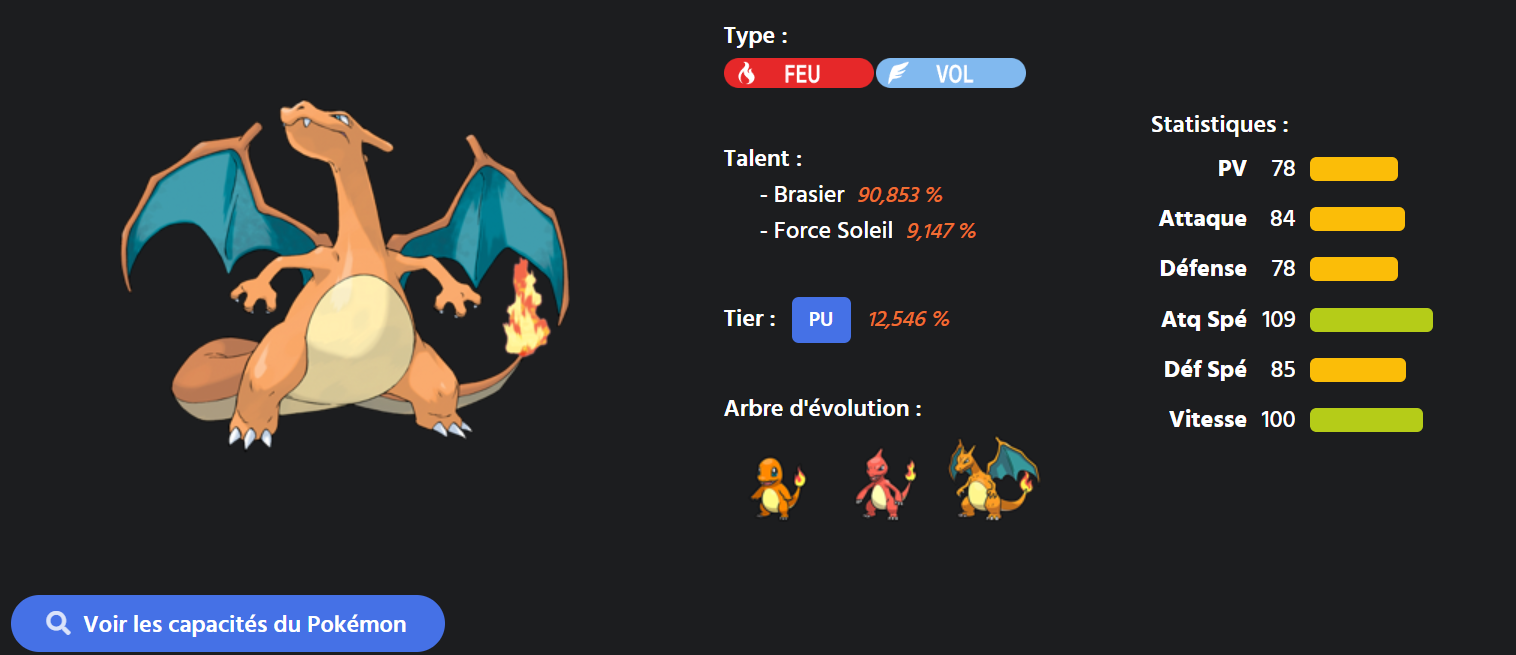
\includegraphics[width=0.6\textwidth]{Image/dracaufeu_coup_critique.png}
    \caption{Page du site coupcritique.fr (site d'analyse stratégique), dédiée à
    Dracaufeu. On y retrouve immédiatement les données citées précédemment)}.
    \label{fig:image1}
\end{figure}

Une explication rapide du déroulement d'une partie s'impose (certains points,
non essentiels à la compréhension, seront passés):
\begin{enumerate}
    \item Avant le début du combat, chaque joueur choisit sont équipes d'au plus
    6 pokémons (en général 6, puisqu'il n'y a aucun intéret à en jouer moins).
    Il choisit pour chaque pokémon leurs capacités parmis celles que le pokémon
    peut apprendre (au minimum 1 et maximum 4, en général 4 car il n'y a pas
    d'avantage à en jouer moins) et leur talent (s'il en ont plusieurs
    disponibles, il faut en choisir un).
    \item Au début du combat, chaque joueur sélectionne le premier pokémon à
    être envoyé sur le terrain.
    \item L'objectif du match est d'amené les points de vie (noté PV ou HP pour
    \textit{Health Points}) de chacun des pokémons de l'adversaire à 0. Chaque
    tour, chaque joueur doit choisir d'executer une des 4 capacités de son
    pokémon, ou de changer son pokémon actif pour un autre de ses 6 pokémons (ce
    qu'on appelle \textit{switch}). Le joueur agissant en premier est déterminé
    à la fois par la statistique de vitesse des pokémons actifs et un système de
    "priorité" (qu'on ne détaillera pas, même si celui-ci se limite en général
    au fait qu'un changement de pokémon se fait avant n'importe quelle capacité
    de l'adversaire). Les capacités peuvent avoir divers effets, mais 3
    catégories sont importantes à retenir :
          \begin{itemize}
              \item les capacités "physiques", qui font baisser les points de
              vie du pokémon adverse en fonction de la "puissance" de la
              capacité (appelée \textit{base power}, propre à la capacité), des
              types de la capacité, du lanceur et de l'adversaire, et des
              statistiques respectivement d'attaque du lanceur et de défense de
              l'adversaire
              \item les capacités "spéciales", semblablent aux capacités
              physiques mais qui se basent sur les statistiques d'attaque
              spéciale du lanceur et de défense spéciale de l'adversaire.
              \item les capacités "de statut", qui provoquent d'autres effets et
              ne se basent sur aucune statistique en particulier.
          \end{itemize}
\end{enumerate}

\begin{figure}[!h]
    \centering
    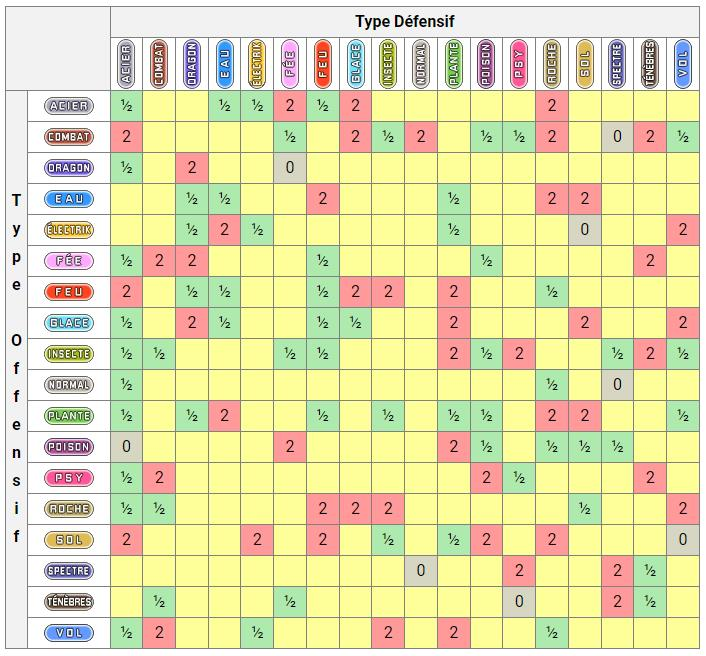
\includegraphics[width=0.6\textwidth]{Image/table-des-types-pour-pokemon-arceus.jpg}
    \caption{Table des types, donnant les modificateurs sur les dégâts infligés
    par une capacité physique ou spéciale en fonction du type de l'attaque et de
    l'adversaire. Ainsi, une capacité de type Feu infligera 2x plus de dégâts
    sur un pokémon de type Plante, tandis qu'elle infligera 2x moins de dégats
    sur un pokémon de type Eau.}.
    \label{fig:image4}
\end{figure}

Les dégâts infligés par les attaques physiques ou spéciales sont calculés via la
formule suivante (version simplifiée) :
\begin{equation}
    PV_{perdus}=\lfloor ( \lfloor \frac{\lfloor \frac{\lfloor 100*0.4+2 \rfloor * Atk * BasePower}{Def}\rfloor}{50}\rfloor +2)*CM \rfloor
\end{equation}
Avec :
\begin{itemize}
    \item $Atk$ la statistique offensive du lanceur (respectivement l'attaque
    pour une capacité physique, l'attaque spéciale pour une capacité spéciale)
    \item $Def$ la statistique défensive du pokémon adverse (respectivement la
    défense pour une capacité physique, la défense spéciale pour une capacité
    spéciale)
    \item $BasePower$ la puissance de la capacité
    \item $CM$ un coefficient comprenant les modificateurs liés aux interactions
    de type (voir la table~\ref{fig:image3}), le \textit{STAB} (modificateur
    augmentant la puissance d'une capacité ayant le même type que son lanceur),
    un potentiel Coup Critique (augmentation aléatoire des dégats)...
\end{itemize}

Ce qu'il faut retenir :
\begin{itemize}
    \item Les statistiques d'attaque et d'attaque spéciale (qu'on notera Atk et
    Sp.Atk) influt positivement sur les dégats infligés par les capacités
    physiques ou spéciales lancées par le pokémon
    \item Les statistiques de défense et de défense spéciale (qu'on notera Def
    et Sp.Def) réduit les dégats reçus lorsque le pokémon subit une capacité
    physique ou spéciale.
    \item La statistique de point de vie (qu'on notera HP) donne le nombre de
    point de vie d'un pokémon au début du combat (qui représente sa capacité à
    encaisser des capacités).
    \item La statistique de vitesse donne l'ordre des actions au sein d'un tour
    (quel pokémon va executer sa capacité en premier).
\end{itemize}

Notons que certaines données influant rarement sur les combats, comme le sexe
des pokémons ou leur poids, ne seront pas pris en compte, car leur influence sur
la viabilité d'un pokémon est négligeable.

\subsection{Présentation du jeu de donnée}
Le tableau \textit{Pokemon.csv} contient, pour chaque pokémon, ses statistiques,
ses types, sa génération d'origine et un attribut "Can Evolve", qui indique si
le pokémon peut encore évoluer ou non (les pokémons utilisés en compétitions
sont, sauf exceptions, entièrement évolués). Il contient donc une partie des
données définissant la viabilité d'un pokémon.

Le second jeu de donnée provient du document \textit{gen9ou-0.json} (fourni par
le simulateur \textit{Pokémon Showdown!}). Une rapide explication du format
compétitif joué sur le site est nécessaire afin de comprendre ce document.

Le format compétitif principal, nommé \textit{OU} pour \textit{OverUsed}, est un
format reprenant les combats entre joueurs disponibles dans les jeux pokémons.
La plupart des pokémons sont autorisés, les pokémons bannis sont en général les
pokémons dit \textit{légendaires} (qui font figure d'objectif final de
l'aventure des jeux, et ont des statistiques largement supérieures aux autres
pokémons), et d'autres pokémons bannis via des votes de la communauté de
joueurs. Certaines règles s'appliquent en plus (interdiction de jouer deux fois
le même pokémon, interdiction d'infliger le statut "sommeil" à plus de 1 pokémon
adverse...), et le combat se déroule selon l'explication plus haut. Les joueurs
sont classés via un système d'ELO similaire à celui utilisé pour les échecs.

Le simulateur garde certaines données de chaque partie jouée sur le site et,
chaque mois, fourni ces données collectées sur le mois précédent. Ces données,
contenues dans le document \textit{gen9ou-0}, contiennent notament :
\begin{itemize}
    \item le nombre total de combat joué
    \item le nombre d'occurences de chaque pokémon
    \item le nombre d'occurences de chaque capacité par pokémon
    \item le nombre d'occurences de chaque talent par pokémon
\end{itemize}
Ces données complètent alors des données manquantes de \textit{Pokemon.csv}. On
fera les deux approximations suivantes :
\begin{itemize}
    \item le taux d'utilisation d'un pokémon représente sa viabilité ou
    "puissance"
    \item les seules capacités influant sur la viabilité d'un pokémon sont
    celles ayant déjà été utilisées sur le simulateur (étant donné que le nombre
    de parties jouées est de l'ordre du million, on peut considérer que toutes
    les capacités "utiles" des pokémons ont été utilisées au moins une fois)
\end{itemize}

\section{Description des données}

\section{Analyse exploratoire des données}


\section{Analyse des données}

Notre projet consiste en la caractérisation du phénomnène de powercreep. Tout
d'abord, il faut vérifier qu'il y a réellement un phénomène de powercreep :
c'est à dire que les pokémons des générations récentes sont plus joués (car plus
fort) que les pokémons des générations précédentes. Une façon simple de vérifier
cela est de regarder les statistiques d'usages de chaque pokémon. Il est alors
facile de constater le powercreep : les 4 pokémons les plus utilisés proviennent
de la $9^{e}$ génération, et parmis les 10 pokémons les plus utilisés en
\textit{OU}, 6 proviennent de la $9^{e}$ génération, 3 proviennent de la $8^{e}$
génération et 1 provient de la première génération. Les générations ajoutant un
peu près toutes le même nombre de pokémon, on constate que les nouveaux pokémons
sont souvent plus viables que les anciens.

Maintenant que nous avons vu que le phénomène de powercreep s'appliquait bien
aux jeux pokémons, nous pouvons nous interesser à comment le design des pokémons
a évolué pour provoquer ce power creep.

La façon la plus simple qu'aurait Game Freak pour augmenter la puissance des
pokémons des nouvelles générations par rapport aux anciennes serait d'augmenter
le total de statistiques des nouveaux pokémons. En effet, les statistiques des
pokémons sont les seuls données strictement "positive" pour un pokémon :  un
type donnent les résistances mais aussi les faiblesses d'un pokémon, tandis que
les talents sont très divers et donc parfois difficilement comparable (un talent
améliore souvent certains aspects par rapport à d'autres).

Ci-dessous se trouve l'évolutions des moyennes sur les générations d'aparition
des statistiques des pokémons, ainsi que leur total de statistique :

\begin{figure}[!h]
    \centering
    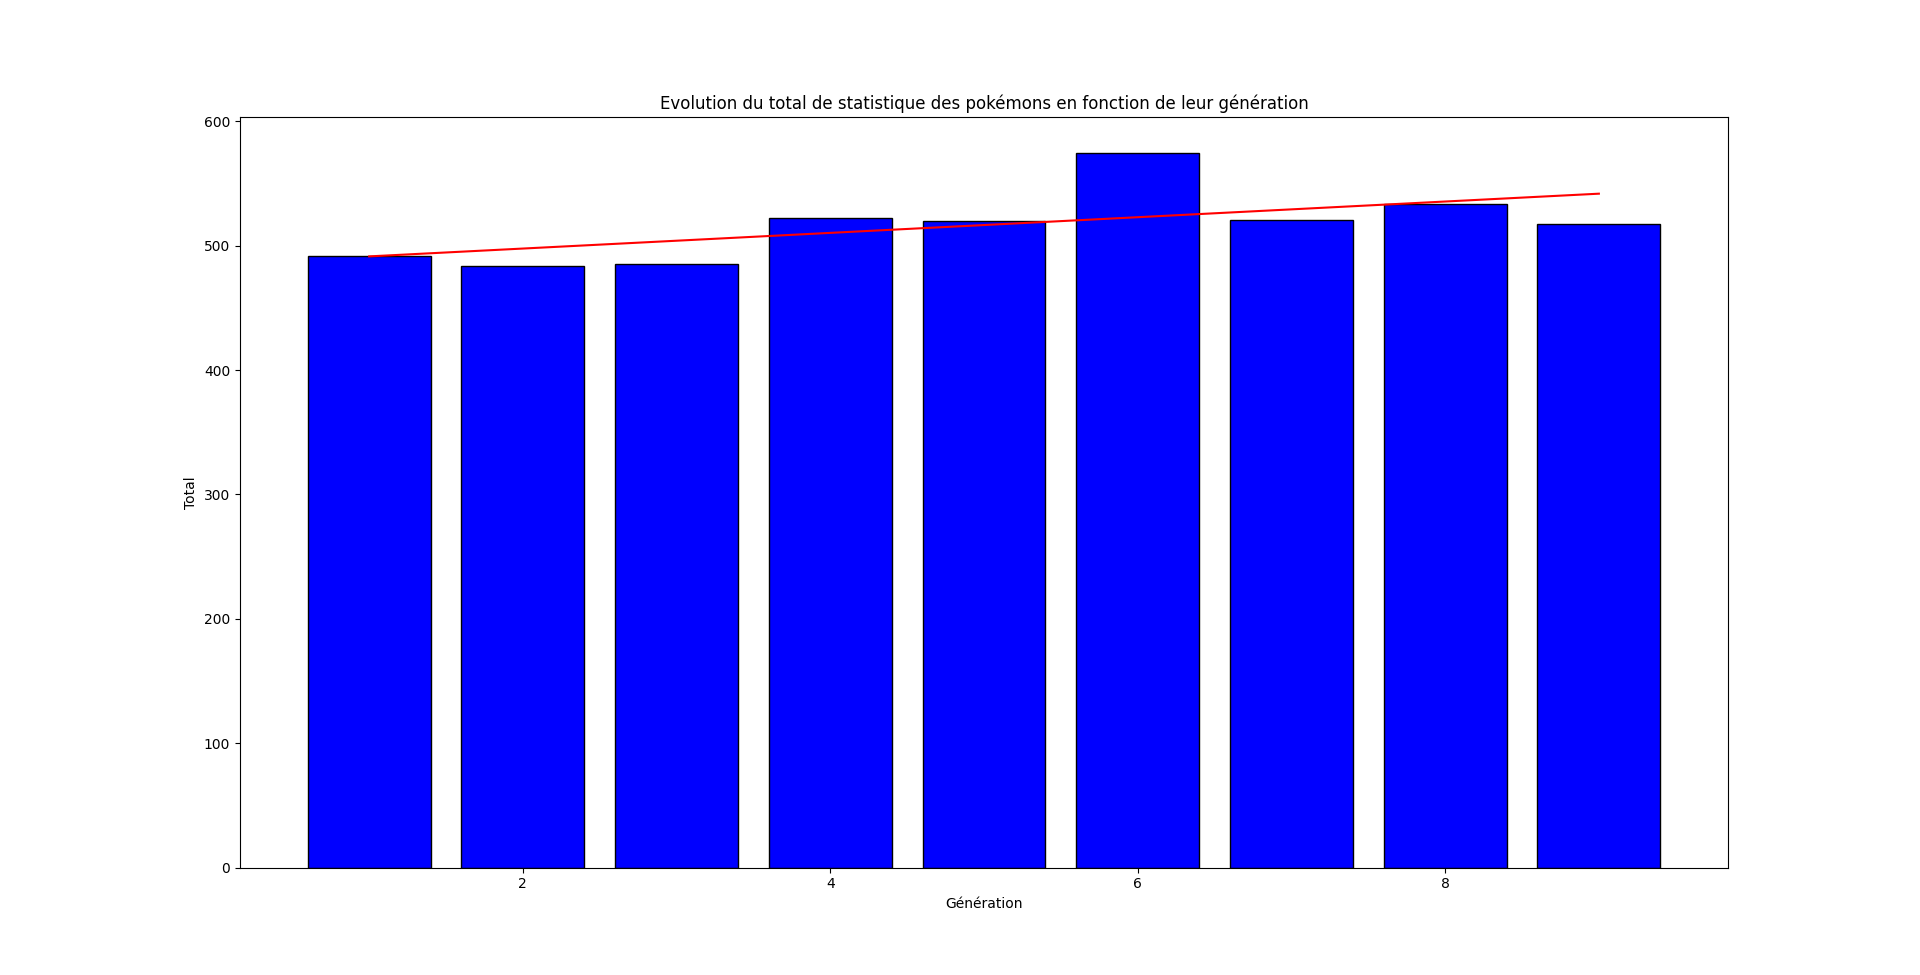
\includegraphics[width=0.95\textwidth]{Image/Total_avg.png}
    \caption{Évolution du total de statistique moyen en fonction de la
    génération}.
    \label{fig:image3}
\end{figure}

\begin{figure}[!h]
    \centering

    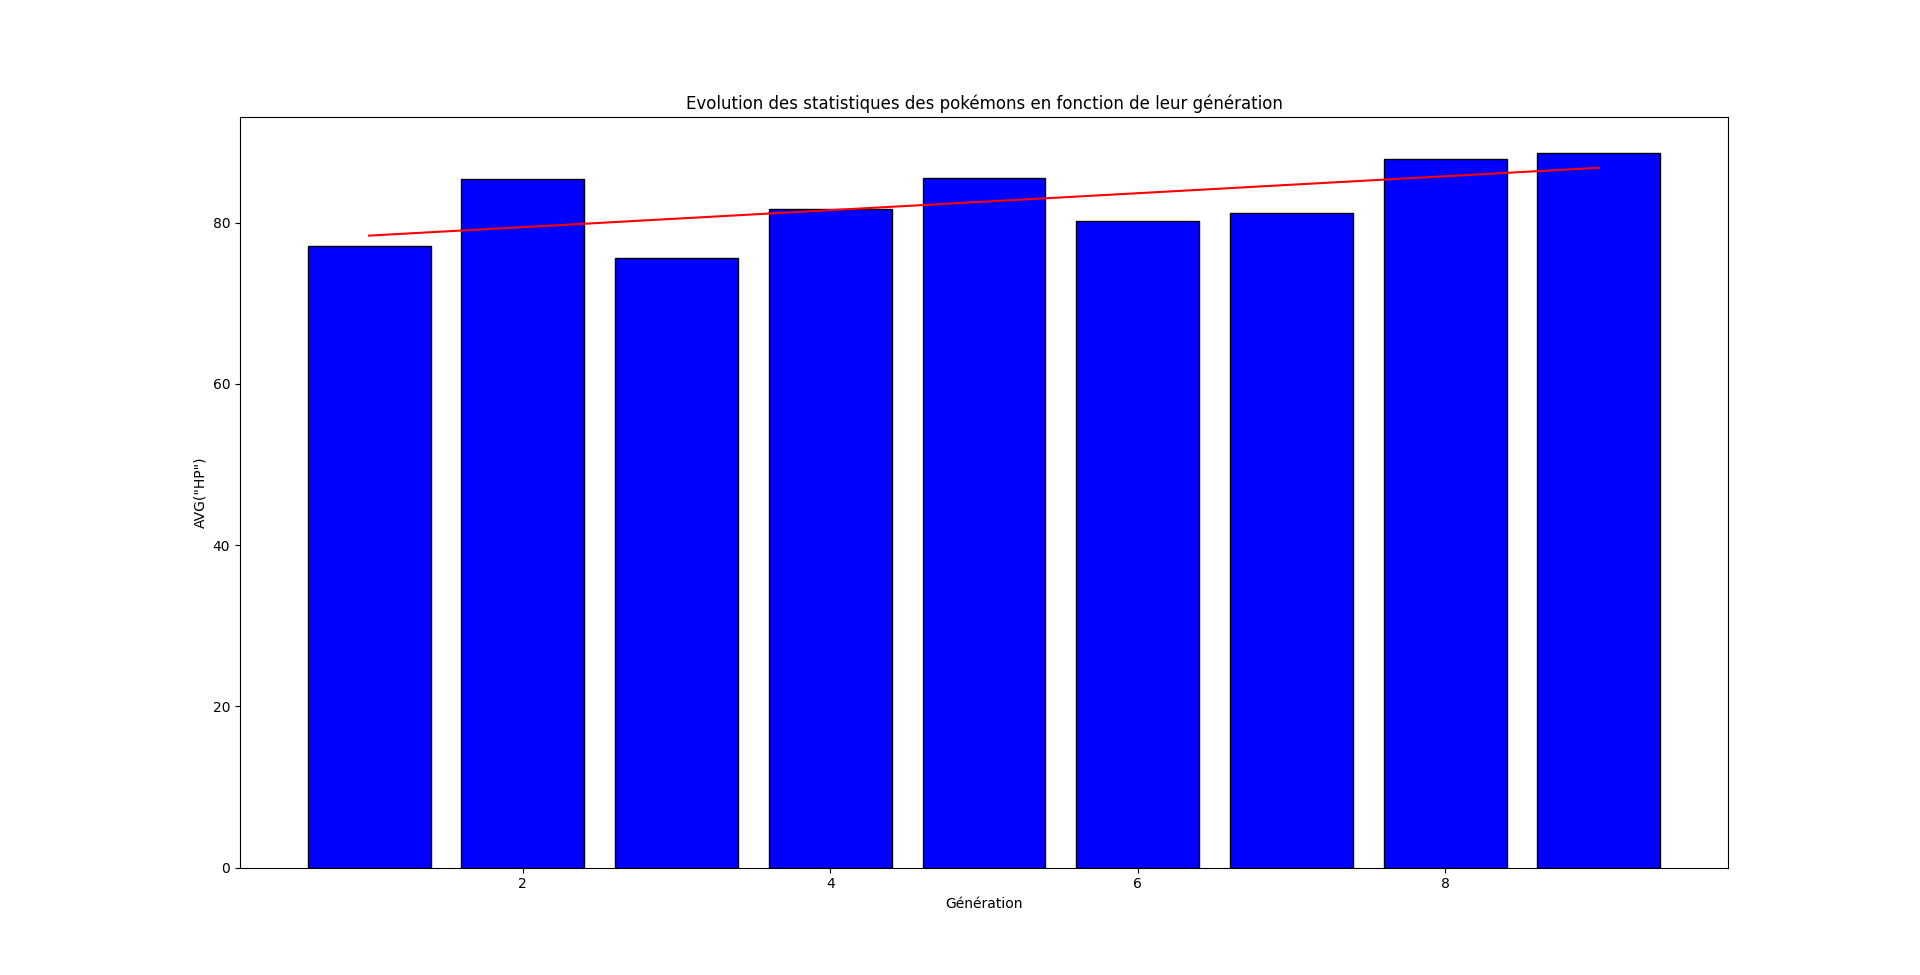
\includegraphics[width=0.3\textwidth]{Image/hp_avg.png}
    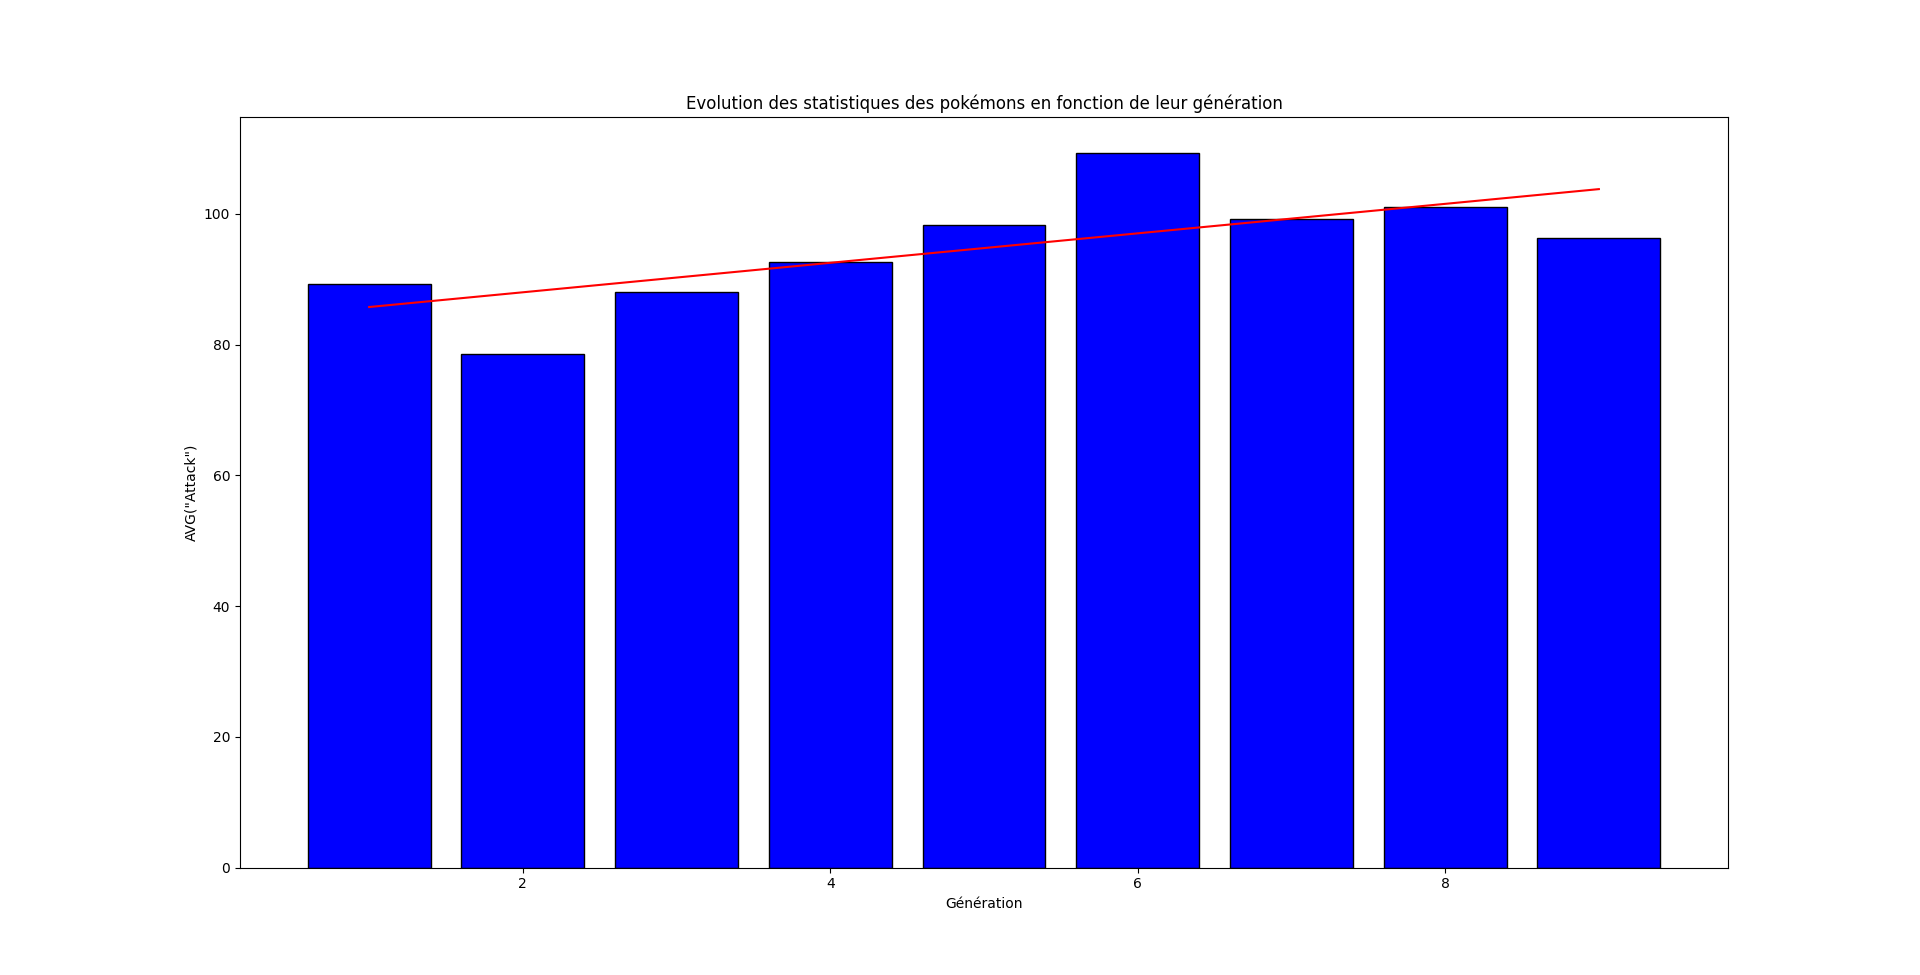
\includegraphics[width=0.3\textwidth]{Image/atk_avg.png}
    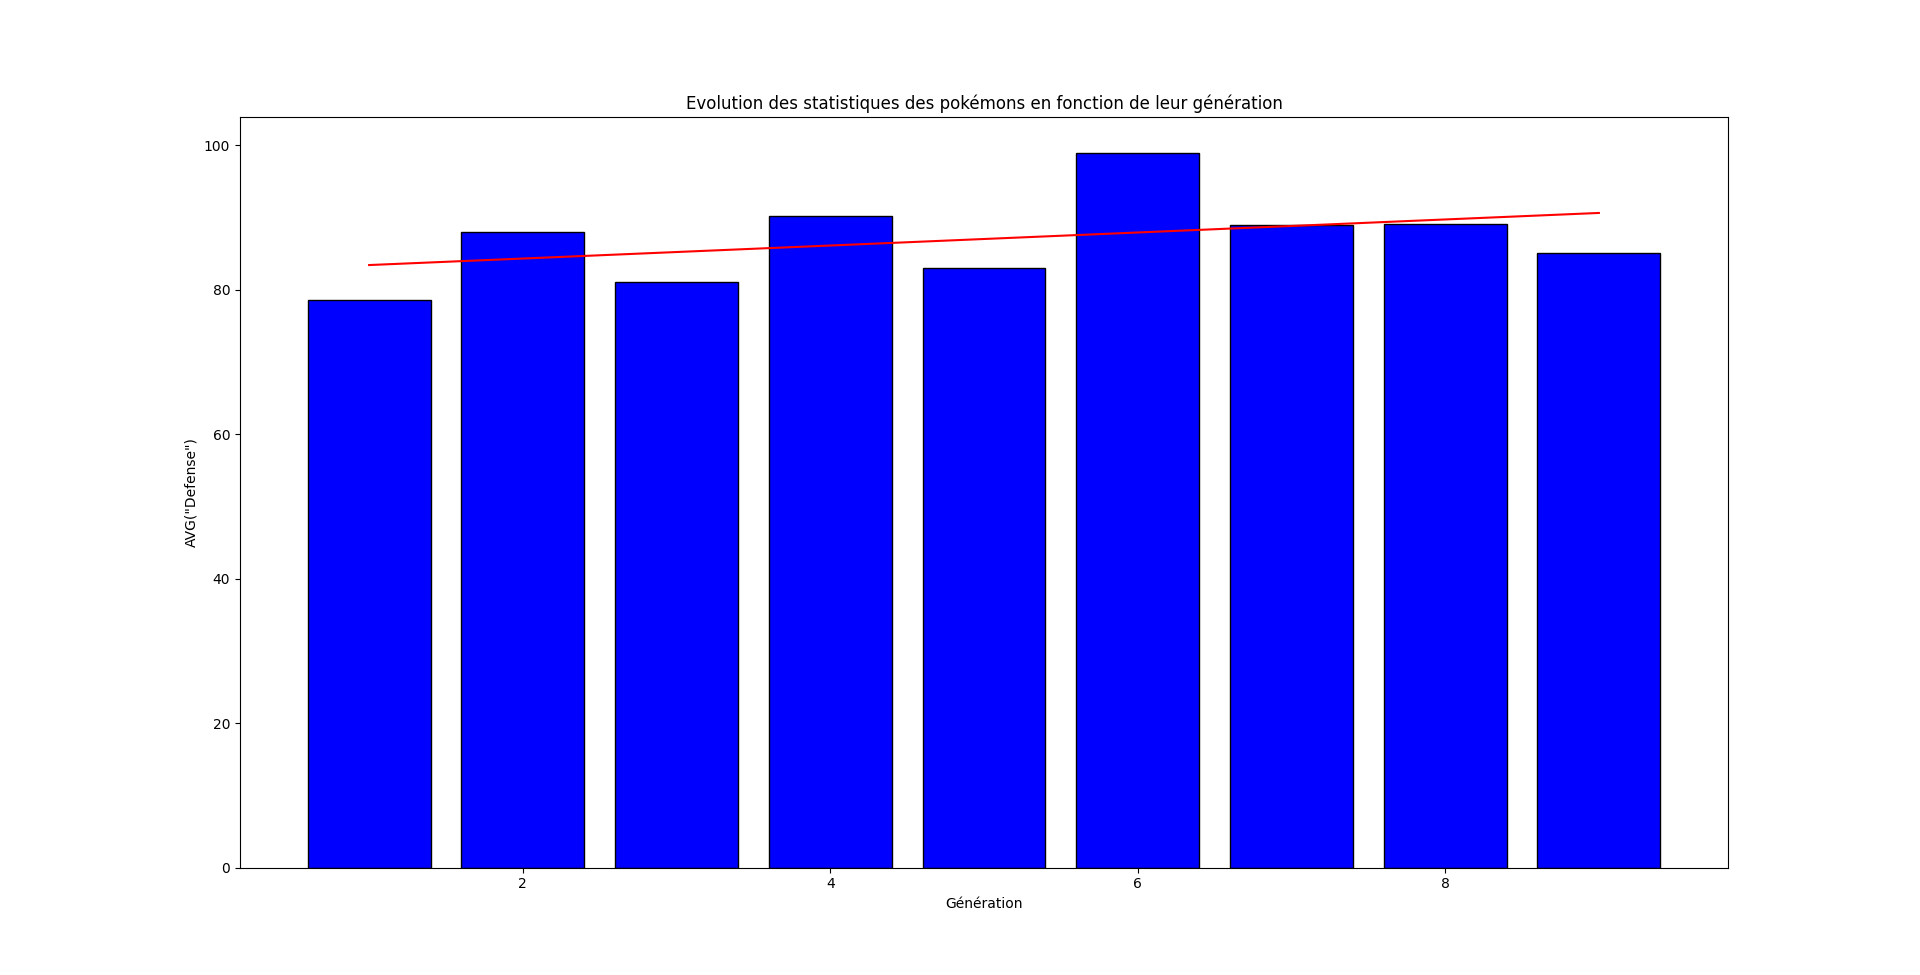
\includegraphics[width=0.3\textwidth]{Image/def_avg.png}

    \vspace{1em}  % Ajoute un espace vertical entre les lignes

    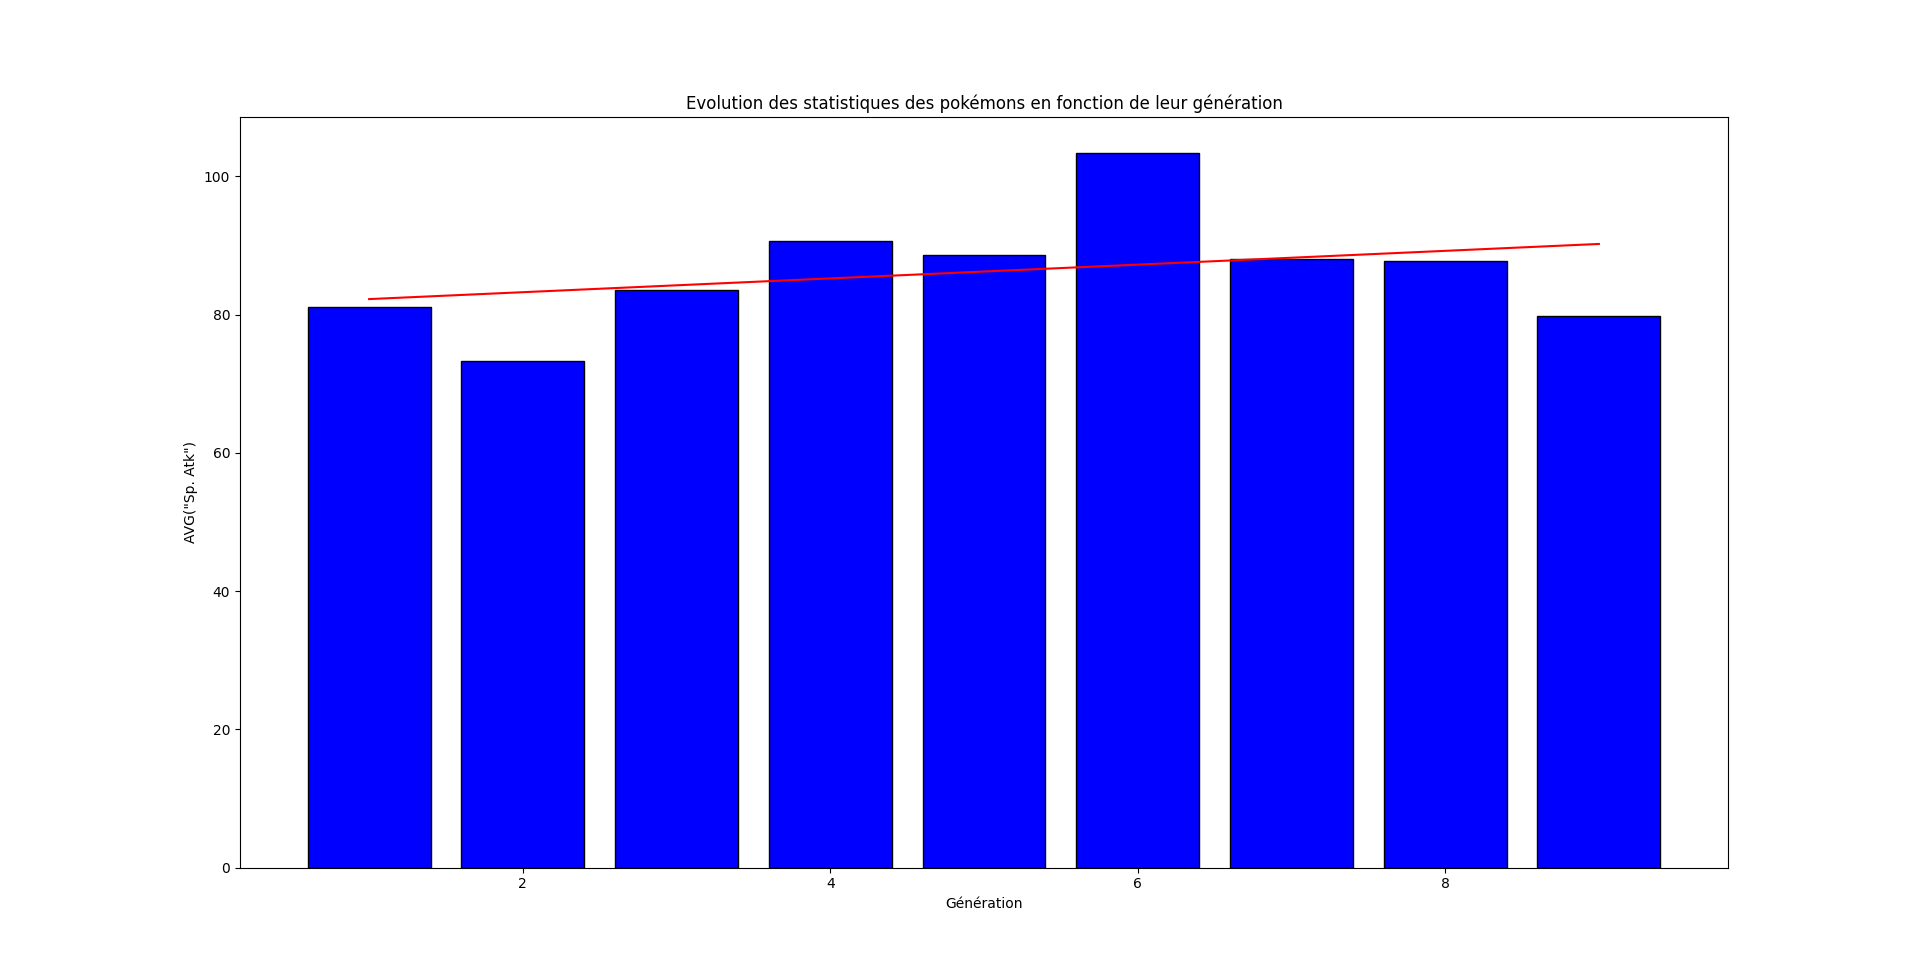
\includegraphics[width=0.3\textwidth]{Image/spatk_avg.png}
    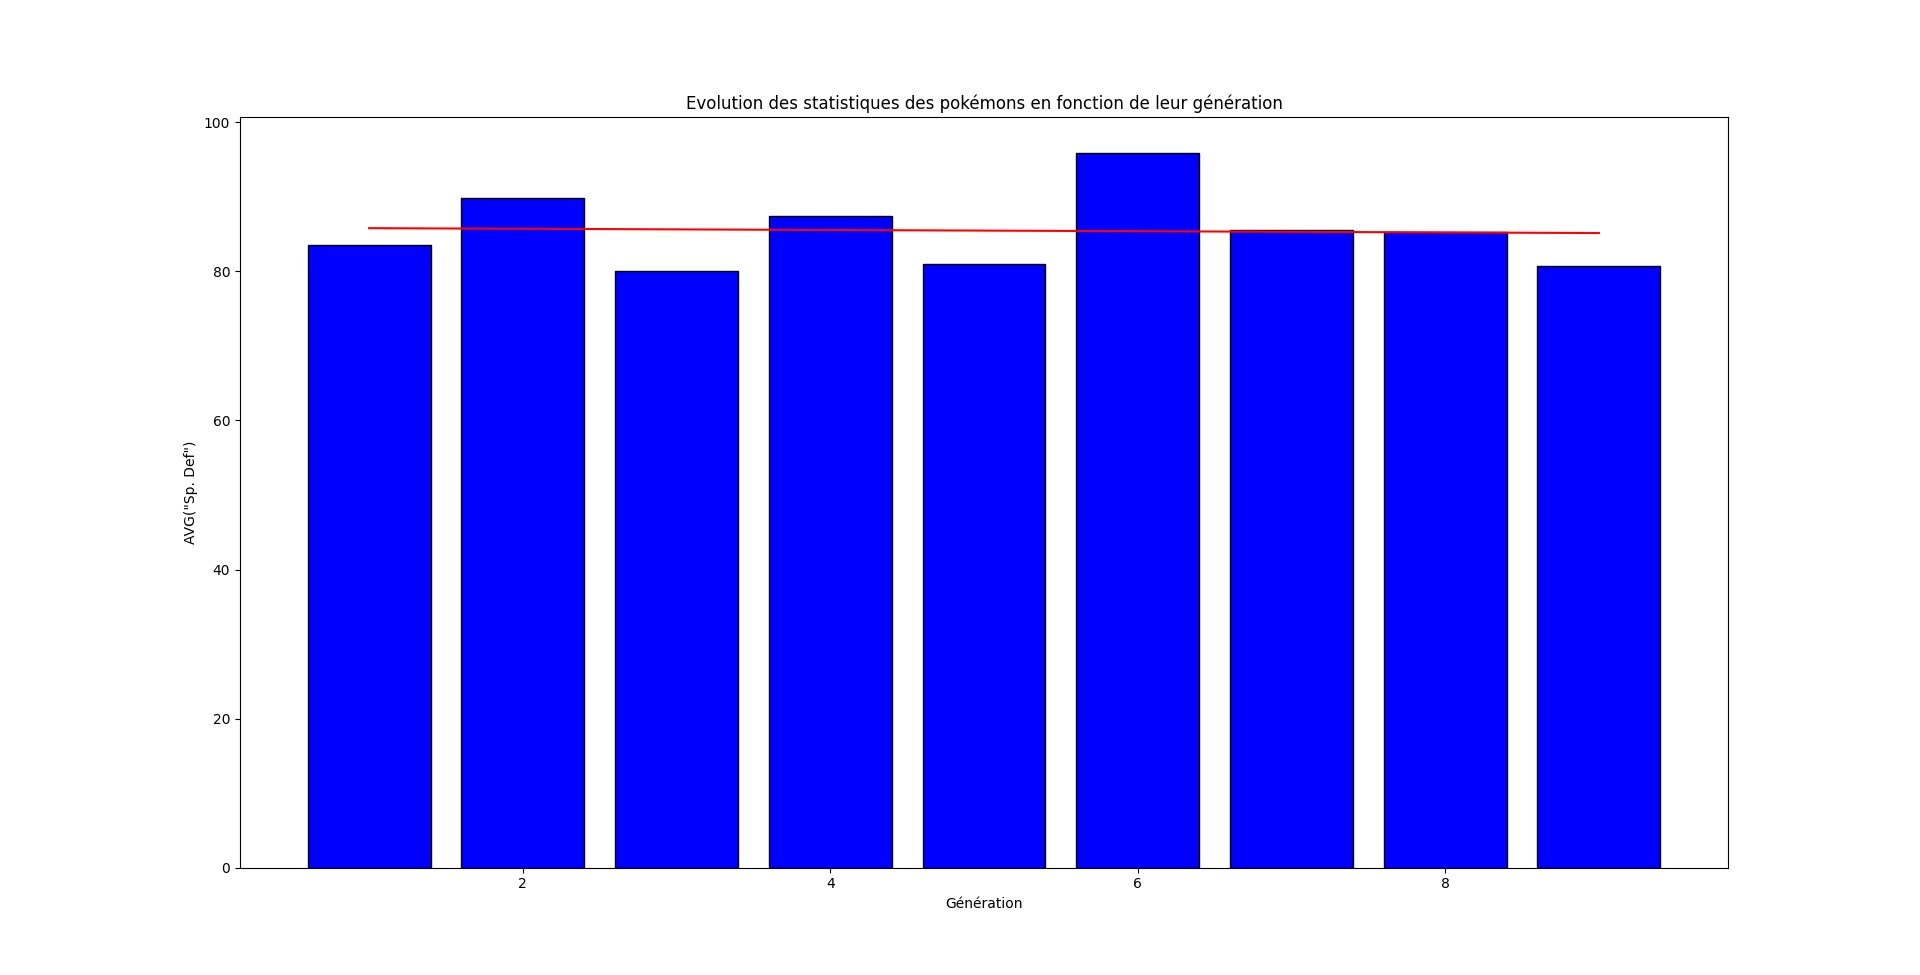
\includegraphics[width=0.3\textwidth]{Image/spdef_avg.png}
    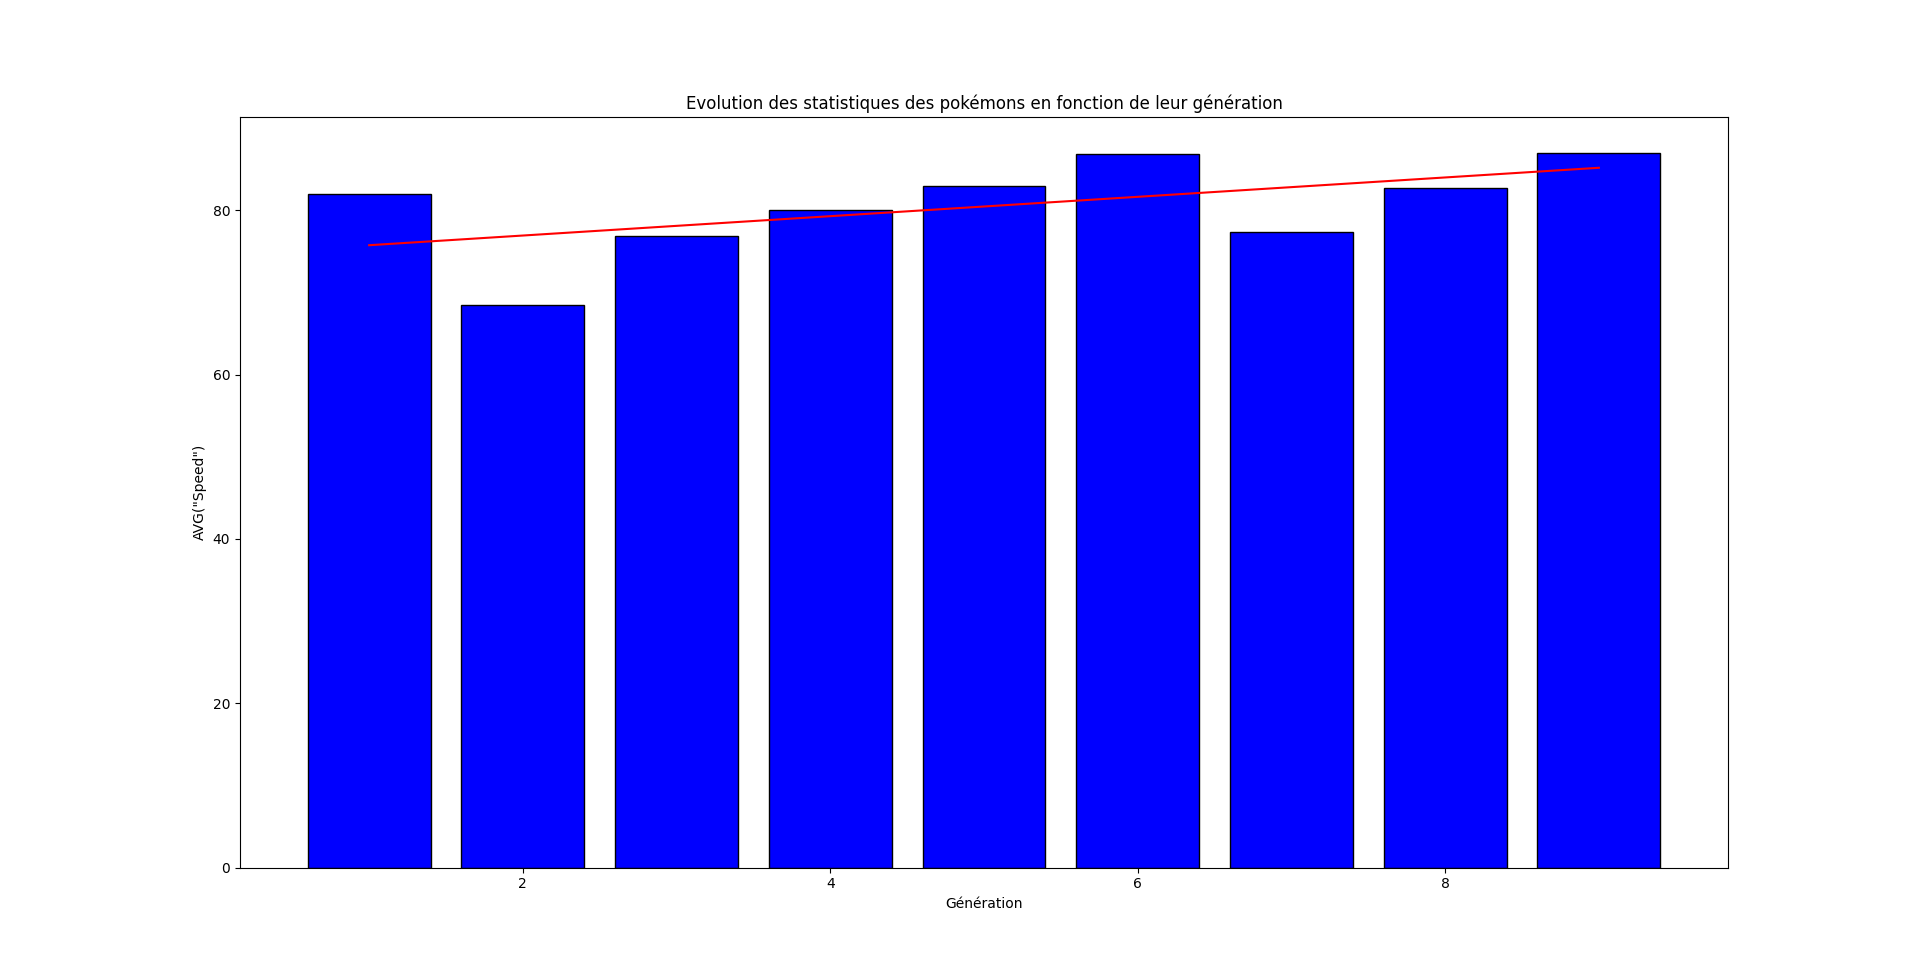
\includegraphics[width=0.3\textwidth]{Image/speed_avg_2.png}

    \caption{Évolution des moyennes des autres statistiques en fonction de la génération}
\end{figure}
\newpage
On peut voir que le total de statistique moyen des pokémons, s'il évolue
positivement avec les générations, n'explique pas seul la prévalence de certains
pokémons, en particulier pour la génération 9 (qui a un total de statistique
moyen inférieur aux générations précédentes).

La suite de notre étude explorera, entre autre, les pistes suivantes :
\begin{itemize}
    \item Impact du movepool sur la viabilité : Quelle est influence de l'accès
    à certaines capacités sur la viabilité des pokémons ? Dans quelle mesure le
    powercreep s'illustre dans l'évolution des movepools ?
    \item Impact du talent sur la viabilité : Quelle est influence de l'accès à
    certains talents sur la viabilité des pokémons ? Dans quelle mesure le
    powercreep s'illustre dans l'évolution des talents ?
    \item Répartition de statistique : Dans la mesure où chaque pokémon joue un
    rôle spécifique dans une équipe, toutes les statistiques d'un pokémon n'ont
    pas la même importance (un pokémon offensif cherchera à agir en premier et
    infliger beaucoup de dégâts, ses statistiques défensives auront donc moins
    d'importance que ses statistiques offensives). Dans quelle mesure les
    répartitions de statistiques équilibrées (dite \textit{fat}) des premières
    générations ont laissé place à des répartitions plus spécialisées ?
    \item Choix des types : Y a-t-il une évolution dans les types des nouveaux
    pokémons ? Celle-ci influt-elle sur la viabilité ?
\end{itemize}

Enfin, nous pourrons nous intéresser aux limites de notre raisonnement (notion
de \textit{metagame}, mécaniques spécifiques à certaines générations, objets...)
et chercher à construire un outil prédictif pour créer de nouveaux pokémons à
partir de statistiques, de types...


\end{document}
